\section{Background}
\label{section:background}

%The abstraction of the overlay network has been proposed as a way to implement
%efficient, fully distributed, application-layer services such as  
%routing messages to destinations that are not known in advance or building
%one-to-many addressing schemes 
% TODO find citation for Narada & Adobe's Real Time Media Flow Protocol (RTMFP)
%\cite{} that provide quality-of-service (QoS) guarantees. \emph{IP
%multicast}, as well as other proposals such as \emph{IntServ} and
%\emph{DiffServ} \cite{cisco_diffserv_2005}, have still not seen wide deployment
%largely due to the fact they require support from the IP
%infrastructure. On the other hand, an overlay network can be deployed on
%end-systems running the overlay protocol software, without the cooperation of ISPs.
%Academic research includes
%\cite{chu_esm_2000,jannotti_overcast_2000,kwon_tag_2002} among others.

In this section, we provide some background information on the types of
peer-to-peer architectures that have been implemented and deployed. We also
describe and motivate more formally the topology mismatch problem tackled by
many P2P researchers over the past several years.

%%%%%%%%%%%%%%%%%%%%%%%%%%%%%%%%%%%%%%%%%%%%%%%%%%%%%%%%%%%%%%%%%%%%%%%%%%%%%%%%
%%%%%%%%%%%%%%%%%%%%%%%%%%%%%%%%%%%%%%%%%%%%%%%%%%%%%%%%%%%%%%%%%%%%%%%%%%%%%%%%
\subsection{Peer-to-Peer (P2P) Overlay Architectures}
%%%%%%%%%%%%%%%%%%%%%%%%%%%%%%%%%%%%%%%%%%%%%%%%%%%%%%%%%%%%%%%%%%%%%%%%%%%%%%%%
%%%%%%%%%%%%%%%%%%%%%%%%%%%%%%%%%%%%%%%%%%%%%%%%%%%%%%%%%%%%%%%%%%%%%%%%%%%%%%%%
Circa 2000, the first P2P file-sharing systems introduced the \emph{servent}
concept \cite{gnutella}, a \emph{portmanteau} that blends the notions of server
and client to denote the twofold role of a node participating in the P2P
network. Such serverless systems have proven to be able to achieve outstanding
aggregate resource capacities as more and more participants join the system
without requiring additional expenditure for infrastructure. While certain
undesirable features such as 
free-riding~\cite{saroiu_measurefileshare_2002,adar_gnutellafreeriders_2000,hughes_gnutellafreeride_2005},
the distribution of illegal content and other \emph{socio-technical}
issues \cite{hughes_socp2p_2008}, have arisen, peer-to-peer systems have
continued to gain popularity mainly because they have successfully supported
popular applications (i.e. file-sharing) amongst vast numbers of participating
users.

For over a decade, excitement over the immense potential of P2P systems has
generated a flurry of research and development, resulting in a wide range of
popular protocols, networks, and applications. As P2P systems evolved, three
main architectures have emerged, namely
\begin{inparaenum}[\itshape i\upshape)]
  \item \emph{centralized},
  \item \emph{decentralized unstructured}, and
  \item \emph{decentralized structured}.
\end{inparaenum}

Designers of \emph{centralized} architectures
(seeFigure~\ref{figure:p2p-archs:centralised}) were the first to recognise that
requests for resources (e.g. CPU cycles or popular content) need
not be sent to a dedicated server but instead could be handled by
the many hosts that already posess the resources. The downside of this approach
is that it requires a centralized searching facility which becomes a single
point of failure, a scalability bottleneck, and a target of malicious attacks
(e.g., \emph{Denial-of-Service (DoS) attacks}).

The most successful incarnation of the centralized approach is the file-sharing
application \emph{Napster}. % TODO find citation for Napster again \cite{}
Napster maintained a \emph{central index server} based on file lists provided by
participating peers. The central index server was queried by users and it
returned pointers to the actual content. Thus, by centralizing search while
distributing downloads, Napster achieved a highly functional design that, at its
height, attracted 26 million users sharing approximately 80 million
songs~\cite{jmm_naptopusage_2001}. Napster's centralized nature was ultimately
what brought it down after Recording Industry Association of America (RIAA) 
filed a lawsuit for copyright infringement of the intellectual property of
artists whose music was distributed by the Napster application. RIAA was able to
point to the centralized indexing component of Napster as the entity responsible
for illegal song-trading.

The centralized approach was quickly replaced by architectures that distribute
both search and resource provision capabilities (see
Figure~\ref{figure:p2p-archs:unstructured-full}). In these \emph{decentralized}
architectures, resource placement within the overlay topology is
random~\cite{YG-M2002}. For this reason they are referred to as
\emph{unstructured}. The most important properties of such systems are that they
support inherent heterogeneity of peers, are highly resilient to peer failures,
and incur low maintenance overhead at handling the dynamics of peer
participation \cite{stutzbach_churn_2006}. In the literature, they are also
known as \emph{broadcast-based} systems, because they use message flooding among
peers to propagate search queries. A well-known example of the fully dentralized
unstructured approach is Gnutella, in its first realisation (v.0.4)
\cite{gnutellav04}.

A key disadvantage of the unstructured approach is that message flooding burdens
the network since queries travel within the network randomly, visiting nodes
that do not have the resource of interest and thus wasting bandwidth.  To save
on bandwidth, unstructured networks typically limit how long a query travels
within the overlay (via a time-to-live (TTL) parameter). When a query is
received by a node, it decreases the TTL by one unit. If the TTL has not reached
zero, the node forwards the query to its neighbours.  Otherwise, it drops the
query. While this approach prevents queries from visiting the entire network, it
does not guarantee that the resource of interest, (e.g., a rare recording 
of a musical group from the 1930s) will be found.

To improve search scope and scalability and to lighten network load, 
unstructured systems evolved into ``hierarchical'' systems that dynamically
assign indexing functions to special peers, called \emph{ultra-peers}  or
\emph{super-peers} (see
Figure~\ref{figure:p2p-archs:unstructured-hierarchical}). Peers with reliable
network connections and/or high compute power became ultra/super-peers
facilitating less powerful peers (called \emph{leaf-nodes}) to find resources of
interest. Well-known examples of these hierarchical unstructured systems include
Gnutella v.0.6/Limewire~\cite{gnutella}, KaZaA~\cite{kazaa} and
Skype~\cite{skype}. While the hierarchical approach relieves network pressure as
search queries are flooded over a much smaller subset of peers (the
ultra/super-peers), the disadvantages of reduced search scope and inability to
locate rare resources efficiently remain.

To fully address the disadvantages of decentralized unstructured approaches,
\emph{decentralized structured} schemes have been proposed (see
Figure~\ref{figure:p2p-archs:structured}). The key goal of these systems is to
provide a self-organising infrastructure for large-scale P2P applications
\cite{ratnasamy_can_2001,stoica_chord_2001,antony_pastry_2001,zhao_tapestry_2001,maymounkov_kademlia_2002,rgrk_bamboo_2004}.
They implement a \emph{Distributed Hash Table (DHT)} that maps objects to nodes
through a deterministic mechanism. The DHT provides a guaranteed bound on the
number of overlay routing hops that have to be taken to locate a resource, even
in the case when only a single copy exists in the system.  This means
$O \left( log n \right)$ hops, compared to unstructured networks that require
$O \left( n \right)$ to reliably locate any object. Unfortunately this
efficiency does not come without cost. Structured overlays can only support
exact-match queries (i.e., queries that identify resources by name) as opposed
to content-based retrieval provided by unstructured overlays. This means
that unstructured overlays can support more versatile resource location queries
such as keyword and partial matching searches. Several popular file-sharing
peer-to-peer applications have been based on DHTs including
Overnet/eDonkey~\cite{overnet}, Kademlia/Kad
Network~\cite{maymounkov_kademlia_2002}, some flavors of
BitTorrent~\cite{c_bittorrent_2003}, and many more.  Moreover, DHTs have sparked
a flurry of research activity and development for a large range of applications:
from distributed search engines to event notification infrastructures to
cloud-based platforms.We cite several examples in the Introduction.

% TODO: Change these pictures to match look-n-feel
\begin{figure}[ht]
\centering
\subfigure[Centralised (SETI@Home or Napster).] {
  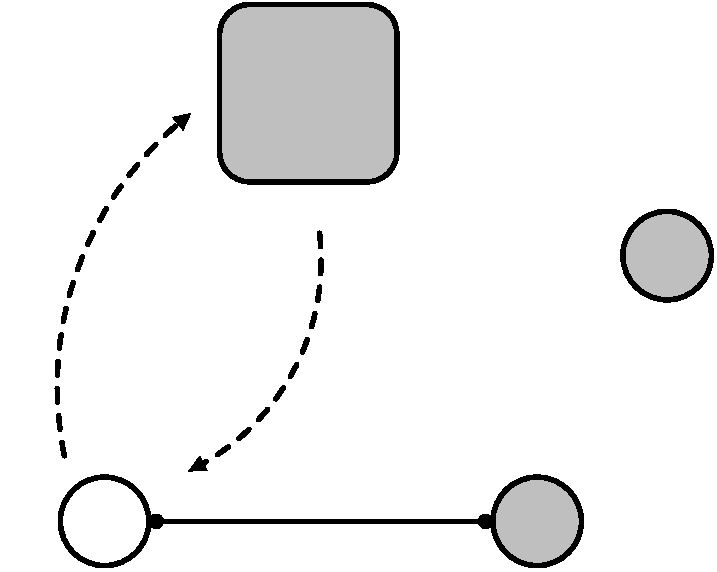
\includegraphics[scale=0.25]{img/pdf/centralised.pdf}
  \label{figure:p2p-archs:centralised}
}\qquad\qquad
\subfigure[Fully unstructured (Gnutella v.0.4).] {
  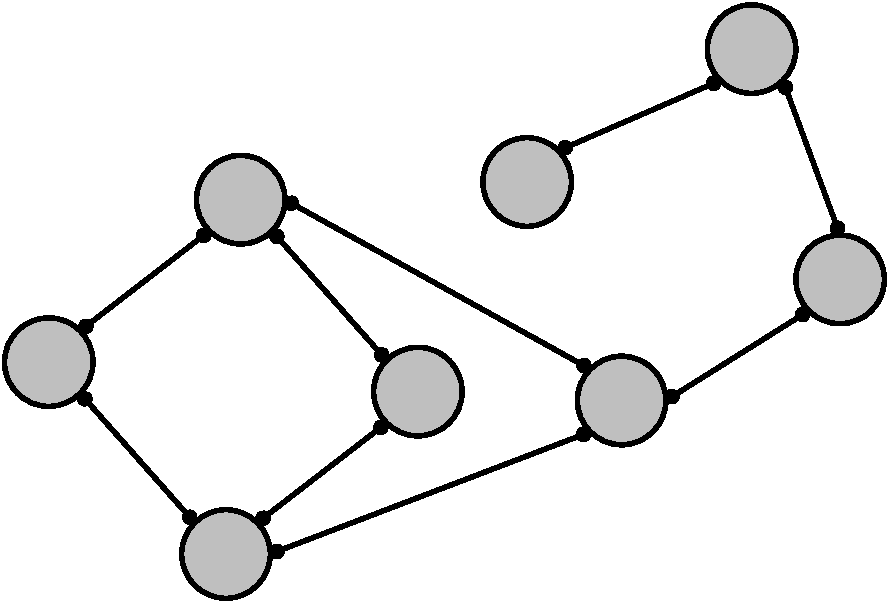
\includegraphics[scale=0.25]{img/pdf/unstructured-full.pdf}
  \label{figure:p2p-archs:unstructred-full}
}\qquad\qquad
\subfigure[Hierarchical unstructured (Gnutella v.0.6 or FastTrack).] {
  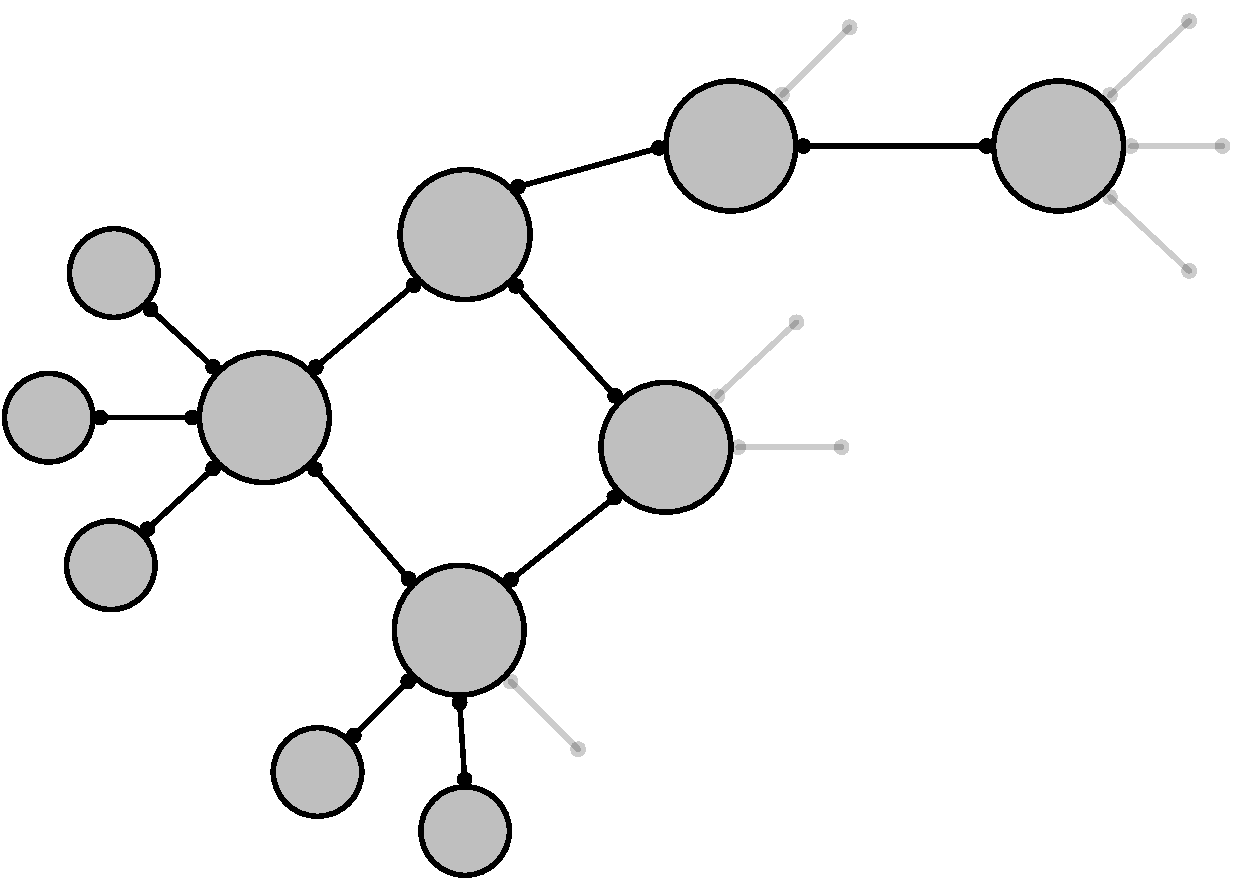
\includegraphics[scale=0.25]{img/pdf/unstructured-hierarchical.pdf}
  \label{figure:p2p-archs:unstructured-hierarchical}
}\qquad\qquad
\subfigure[Structured (Chord and Kademlia).] {
  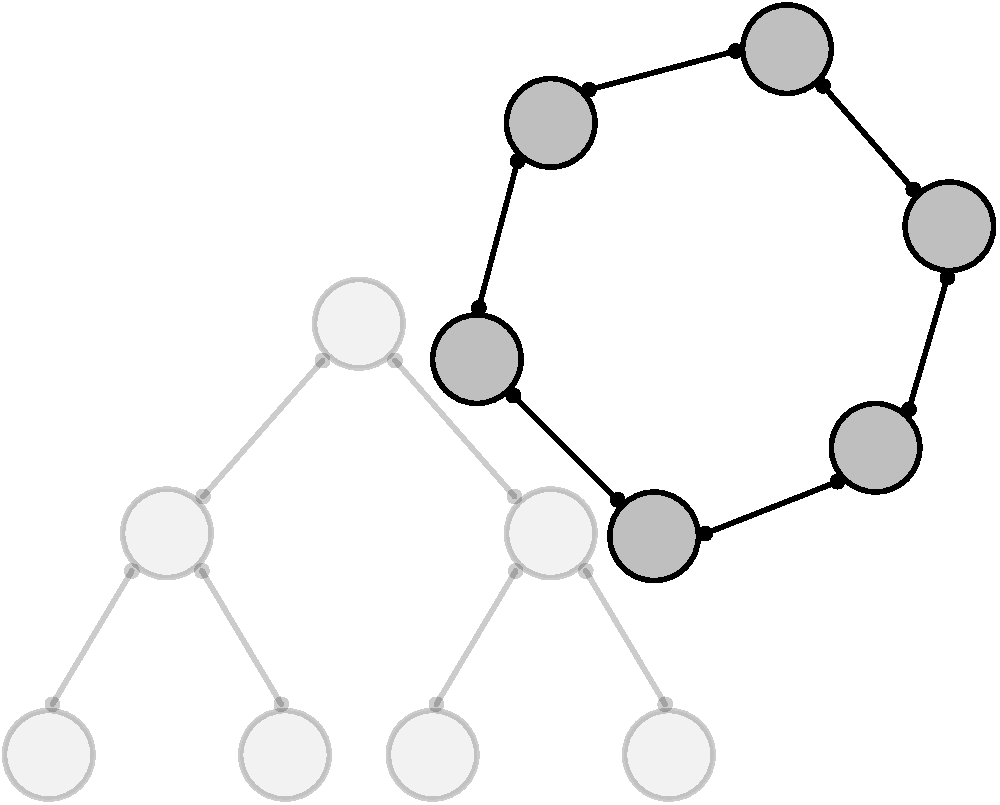
\includegraphics[scale=0.25]{img/pdf/structured.pdf}
  \label{figure:p2p-archs:structured}
}
\caption{The various peer-to-peer architectures.}
\label{figure:p2p-archs}
\end{figure}

%%%%%%%%%%%%%%%%%%%%%%%%%%%%%%%%%%%%%%%%%%%%%%%%%%%%%%%%%%%%%%%%%%%%%%%%%%%%%%%%
%
% TODO: SOME DISCUSSION ON P2P ARCHITECTURES
%
%\cite{matei_mapgnutella_2002, lv_randomwalks_2002, merugu_str2unstr_2003}
%showed that the ad-hoc network topology of unstructured overlay networks that
%preserve \emph{Power Law} and \emph{Small World} characteristics\footnote{Power
%Law describes the node degree while the Small World describes characteristics
%of path length and clustering coefficient. The clustering coefficient for a
%node $\upsilon$ in a graph $G = \left( V, E \right)$ is defined as the ratio of
%the existing connections between $\upsilon$'s neighbouring nodes to $\gamma
%\times \left( \gamma - 1 \right)$, where $\gamma$ is the number of neighbouring
%nodes of $\upsilon$. High cluster coefficient means that neighbouring nodes of
%any node $\upsilon$ likely connect one another.} \cite{faloutsos_powerlaw_1999,
%saroiu_measurefileshare_2002} offer a more promising approach. Particularly:
%\begin{itemize}
%  \item Peer-to-peer clients are extremely \emph{transient}. Unstructured
%systems can have high maintenance traffic in delivering messages, updating the
%mapping, discovering failures and replicating lost data or pointers, making
%them insufficient on highly volatile networks.
%  \item \emph{Keyword searches} versus \emph{exact-match queries}. In DHTs
%there is a tight control between the data placement and the topology of the
%network. For this reason it is hard to efficiently support partially matched
%queries while Gnutella and other similar systems effortlessly support keyword
%searches and other complex queries since the mechanism is realized locally, on
%a node-by-node basis.
%  \item Popular content is located at multiple peers and thus it is more likely
%for a flooding-based search to return results. DHTs, on the other hand, fit
%better in the systems which require ability to reliably locate content, even in
%the extreme case that only a single-copy exists in the network.
%\end{itemize}

%
% TODO: SOME DISCUSSION ON THE ADVANTAGES OF UNSTRUCTURED NETWORKS FROM
%       \cite{z-yk_ddno_2005}
%
%Unstructured P2P networks o?er a number of
%important advantages: (i) An unstructured network
%imposes very small demands on individual nodes,
%and more speci?cally it allows nodes to join or leave
%the network without signi?cantly a?ecting the sys-
%tem performance. (ii) Unstructured networks are
%appropriate for content-based retrieval (e.g., key-
%word searches) as opposed to object identi?er loca-
%tion of structured overlays. (iii) Finally unstructured
%networks can easily accommodate nodes of vary-
%ing power. Consequently, they scale to very large
%sizes and they o?er more robust performance in
%the presence of node failures and connection
%unreliability.
%

%
% TODO: SOME DISCUSSION ON STRUCTURED OVERLAYS PROBABLY FROM
%       \cite{WLH2007}
% However, the design of a decentralized but structured P2P network has to
% overcome two critical issues. The first issue is the long routing latency.
% Several proximity schemes  have been proposed to avert long routing latency in
% current structured P2P networks, but they require a high-complexity procedure
% to periodically maintain the routing table (e.g. Pastry system) or they need
% pre-chosen landmarks to construct the overlay. However, the P2P system is by
% its very nature unstable since nodes join and leave frequently. For instance,
% the study of Gnutella shows around approximately 1200 membership changes per
% minute in a 100 000 nodes P2P system. Another proximity scheme needs some
% pre-chosen landmarks or a complete BGP routing table support. As a result,
% they both increase the difficulty of the P2P system deployment. The second
% issue is system maintenance overhead. The existing structured P2P networks
% allow nodes to keep some nearby nodes in their routing tables in order to
% achieve efficient routing.
%


%%%%%%%%%%%%%%%%%%%%%%%%%%%%%%%%%%%%%%%%%%%%%%%%%%%%%%%%%%%%%%%%%%%%%%%%%%%%%%%%



%%%%%%%%%%%%%%%%%%%%%%%%%%%%%%%%%%%%%%%%%%%%%%%%%%%%%%%%%%%%%%%%%%%%%%%%%%%%%%%%
%%%%%%%%%%%%%%%%%%%%%%%%%%%%%%%%%%%%%%%%%%%%%%%%%%%%%%%%%%%%%%%%%%%%%%%%%%%%%%%%
\subsection{The Topology Mismatch Problem}
%%%%%%%%%%%%%%%%%%%%%%%%%%%%%%%%%%%%%%%%%%%%%%%%%%%%%%%%%%%%%%%%%%%%%%%%%%%%%%%%
%%%%%%%%%%%%%%%%%%%%%%%%%%%%%%%%%%%%%%%%%%%%%%%%%%%%%%%%%%%%%%%%%%%%%%%%%%%%%%%%

One of the major issues that defines the efficiency of an overlay network is the
mapping of the overlay structure to the underlying infrastructure. Remember, in
Figure~\ref{figure:overlay} nodes $A$ and $B$ are on the same local network,
while $C$ and $D$ are in different networks. The top layer represents the
overlay interconnection formed by these nodes at a higher level. Link
connections there, can change as needed by the running environment, without any
particular constraint by the underlying physical topology. Let's have a closer
look with the help of a simple example. Assume nodes $A$, $B$, $C$ and $D$ are
connected through the physical network shown in Figure~\ref{figure:phys}, where
the network costs are given in milliseconds, and peer $A$ sends a message to
peer $D$.

\begin{figure}
\centering
  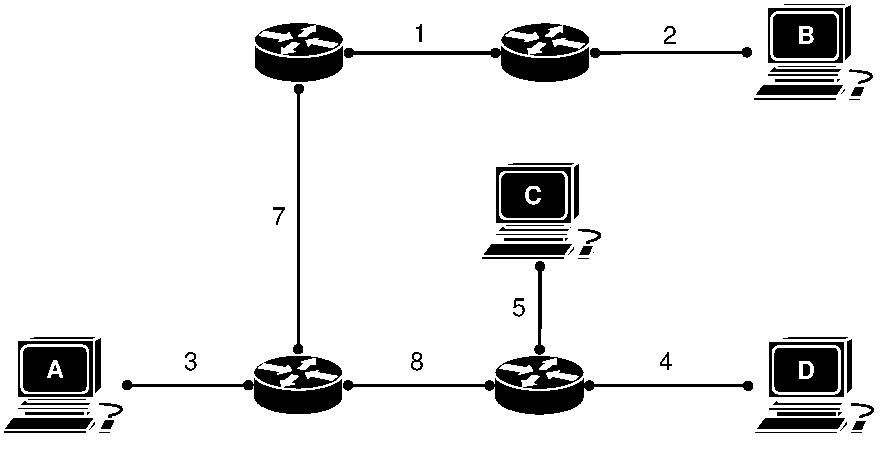
\includegraphics[scale=0.7]{img/pdf/example-physical.pdf}
\caption{Interconnection of nodes in the physical level.}
\label{figure:phys}
\end{figure}

If these peers participate in an overlay network according to one of the setups
of Figure~\ref{figure:overlay-confs}, then users will experience different
performances. In the overlay depicted in Figure~\ref{figure:overlay-1}, the
message will traverse the following sequence of links in the physical layer
(marked with their costs): $3 \rightarrow 7 \rightarrow 1 \rightarrow 2
\rightarrow 2 \rightarrow 1 \rightarrow 7 \rightarrow 8 \rightarrow 5
\rightarrow 5 \rightarrow 4$. In the alternative overlay of
Figure~\ref{figure:overlay-2}, the path will be: $3 \rightarrow 8 \rightarrow
4$. The total cost of the first sequence is $45 ms$, while the second yields a
mere $15 ms$. Therefore, we can conclude that the second overlay is more
congruent with the underlying physical network than the first one and, thus, is
more efficient.

\begin{figure}[ht]
\centering
\subfigure[Nodes B and C have direct overlay connection.] {
  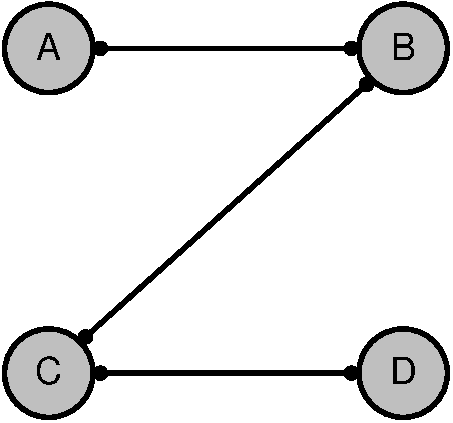
\includegraphics[scale=0.5]{img/pdf/example-overlay-inefficient.pdf}
  \label{figure:overlay-1}
}\qquad\qquad
\subfigure[Nodes A and D have direct overlay connection.] {
  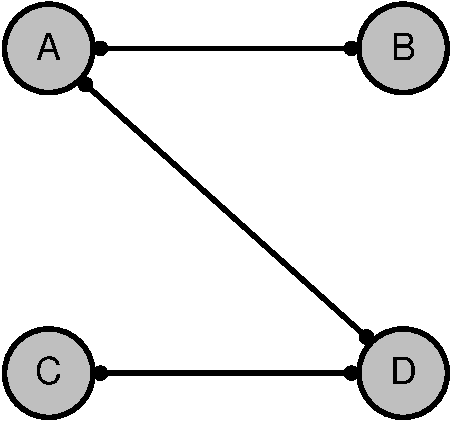
\includegraphics[scale=0.5]{img/pdf/example-overlay-efficient.pdf}
  \label{figure:overlay-2}
}
\caption{Two different overlay connection configuration.}
\label{figure:overlay-confs}
\end{figure}

Ideally, an overlay network should be constructed to achieve an optimal 
mapping among the overlay paths and the underlying IP network links to avoid
inefficient states. The problem of constructing an optimal overlay is referred
to as the \emph{topology mismatch problem}, and is formally defined as follows:
\begin{definition}
Let $V = \{v_1, ..., v_n\}$ be a set of points denoting the network nodes,
$\{v_i, v_j\} \in E$ be the set of unicast distances between nodes $v_i$ and
$v_j$, $G=(V,E)$ be a complete distance graph over $V$. The topology mismatch
problem is to construct a minimal spanning tree, where node degree is
restricted to a constant ($k\geq 2$) by the bandwidth of each node $v_i$.
\end{definition}

Early incarnations of the overlay protocols did not make use of the optimal
mapping with the underlying network topology. Gnutella, for example, is
considered far from scalable \cite{ritter_gnucantscale_2001} because every peer
chooses its neighbors in the overlay without any knowledge of the underlying
network, resulting in a mismatch between the two topologies. Queries may be
flooded over multiple paths merging in one peer while one of the paths would
have been enough. Moreover, peers may forward the same message to each other
before they receive the query messages from each other.
\cite{matei_mapgnutella_2002} showed that, even when 95\% of any two nodes are
less than 7 hops away from each other, a \emph{flooding-based} algorithm, like
the one used by Gnutella, can generate 330TB/month in a 50.000 node network. A
topology mismatch can thus have a serious effect on Internet router performance.

Similar problems are observed in decentralized structured schemes as well.
Typically, node IDs are assigned \emph{randomly}, resulting in excellent load
balancing, scalability, and robustness for the overlay. Unfortunately, this
randomness has a negative impact on the \emph{routing locality} of the network.
This means that even though the target node can be reached with logarithmic
overlay hops, the distance traveled in the underlying network, during the
overlay routing process, can be far from optimal.  The ratio of the actual IP
network distance a query travels to reach an object of interest (via overlay
routing) to the minimal IP network distance to that object (i.e. through IP) is
known as \emph{stretch} or \emph{Relative Delay Penalty (RDP)} \cite{CRZ2000}.

%%%%%%%%%%%%%%%%%%%%%%%%%%%%%%%%%%%%%%%%%%%%%%%%%%%%%%%%%%%%%%%%%%%%%%%%%%%%%%%%
%%%%%%%%%%%%%%%%%%%%%%%%%%%%%%%%%%%%%%%%%%%%%%%%%%%%%%%%%%%%%%%%%%%%%%%%%%%%%%%%
\subsection{Motivation and Goal for this Survey}
%%%%%%%%%%%%%%%%%%%%%%%%%%%%%%%%%%%%%%%%%%%%%%%%%%%%%%%%%%%%%%%%%%%%%%%%%%%%%%%%
%%%%%%%%%%%%%%%%%%%%%%%%%%%%%%%%%%%%%%%%%%%%%%%%%%%%%%%%%%%%%%%%%%%%%%%%%%%%%%%%
A topology unaware overlay network is able to control the sequence of peers a
message traverses before reaching its destination, but it is completely unaware
of how the actual packets are switched at the underlying infrastructure along
the overlay path. For example, a single logical point-to-point link on the
overlay typically corresponds to multiple physical links in the
underlying layer. Additionally, a link in the underlying network often lies
on several overlay paths causing increase of the traffic on the
link, known as the link's \emph{stress}~\cite{CRSZ2002}. Even in the case
of an approach that provides mechanisms to a newcoming node to detect close-by
peers at join time, the stochastic behaviour with which peers join and leave
the overlay network, called the network's churn, further undermines the effort
for maintaing the best position in the network throughout the life-time of a
peer.

The topology mismatch problem is exacerbated by the extremely large amounts of
traffic generated by highly popular P2P applications (refer to the discussion
made in Section~\ref{section:intro}). Thus, solving the topology mismatch
problem is a fundamental challenge in contributing to the overall efficiency of
the Internet. Unfortunately, topology mismatch is known to be an NP-Hard problem
\cite{NPBOOK,chawathe_scattercast_2000}. Adding to the complexity of the problem
is the fact that end-to-end latencies demonstrate \emph{triangle inequality
violations (TIVs)} which are a consequence of the Internet's structure and
routing policies and thus will remain a property of the Internet for the
foreseeable future \cite{zheng_irprtt_2005}. TIVs affect both network coordinate
\cite{cox_vivaldi_2004,wong_meridian_2005} and positioning \cite{ng_gnp_2001}
systems and makes the construction of IP-topology-aware overlays difficult.

Over the past several years, researchers have proposed and studied an extensive
array of heuristic solutions to the topology mismatch problem. The purpose of
this survey is to gather and organize the extensive knowledge that has been
produced. We hope to assist the reader to understand the different approaches
that have been proposed to tackle the topology mismatch problem. In order to do
so, we dedicate a discussion subsection after the presentation of the algorithms
for both unstructred and structured architectures. This section offers:
\begin{inparaenum}[\itshape i\upshape)]
  \item further discussion that can help the reader identify, through
a taxonomy, the pluses and minuses in the preceeding material,
  \item a comprehensive tabular organisation of the key-point information, and
  \item an attempt to give a pictorial comparison of the relative performance of
the algorithms.
\end{inparaenum}

In discussion we offer the reader a deeper insight for the observations that
pushed research toward some direction. Thus, we try to categorise these
approaches so that we can organise directions making them comprehensible
and helping the reader build critical thinking on the advantages and
disadvantages of each approach.

Tables provide a one-stop-shop overview for the algorithms so that can be a
helpful tool both as a companion during reading the survey and a reference for
future use.

Pictorial comparison consists of bar charts that give a relative feeling of the
perfomance of the various algorithms, discussed in the corresponding section, in
terms of \emph{efficiency}, \emph{overhead} and \emph{scalability}; three
important characteristics for every distributed algorithm. For all we used a
coarse grained, three level, gradation to denote how well the algorithms do,
namely \emph{low}, \emph{medium} and \emph{high}. Each category has its own
interpretation of the above literal values. Efficiency means how well the
algorithm performs its search and topology adaptation functions, without
effecting other characteristics of the networks (e.g. BitTorrent's optimal
dowload performace). To name few, we assume that efficieny is
negatively effected when an algorithm reduces the search scope. Moreover, the
minimum-spanning-tree-based tecniques have slow convergence speed in topology
adaptation or the high clustering impacts load balancing and constrains search
scope (or at least increases search satisfaction time), all reducing overall
efficiency. With overhead we track the cost to compute and communicate peer
join, message forwarding and topology maintenance. For example when exchanging
cost tables only along neighbours the traffic generated can be considered
trivial. Also duplicates minimisation is a plus and lazy or heart-beat-based
overlay control mechanisms impose different amount of stress to the network.
Nevertheless, caching/replication helps reducing the averall overhead by
constraining the query from spreading too much. Minimum-spanning-tree-based
approaches's low convergence speed we mentioned above for efficiency means
additional computational and communicational overhead. % TODO: We check
% complexity in the asymptotic sence, using \emph{Big O} notation % in order to
% check how the algorithm responds t. We take into account topology % creation and
% topology maintenance...
% TODO: HELP NEEDED!
With scalability we check the systems behaviour with respect to the number of
participating peers. Low, medium and high scalability can be generally
considered in the order of hundrends, tenths of thousands and millions,
respectivelly. Fully distributed aproaches is a plus (no system-centric entities
involved, no need for global knowledge) and topology adaptation streanghtens
scalability in highly dynamic environments. Reduced search scope, on the other
side, penaltises the scalability since the more peers comming in the network the
more potentially unsatisfied queries there will be. Furthermore, clock
synchonisation is a limiting factor to scalability of a distributed systems.
Again to name a few.

%
% TODO: SOME DISCUSSION FROM \cite{XTZ2003) CONTRADICTS TO THE
%TRIANGLE INEQUALITY ARGUMENT ABOVE
%
%[snip]
%Studies [14] have shown that triangle inequality may not hold in Internet
%topology. In fact, study from Pastry has shown that the proximity approximation
% is much worse when using the Mercator topology that is based on the real
% measurements of the Internet [3].
%

